\documentclass{article}
\usepackage{makeidx}
\usepackage{hyperref}
\usepackage{amsmath}
\usepackage{amssymb}
\usepackage{xcolor}
\usepackage{graphicx}
\usepackage[top=1in, bottom=1in, left=1in, right=1in]{geometry}

\title{Reinforcement Learning Notes}
\author{chtunsw@gmail.com}
\date{}

\makeatletter
\renewcommand\paragraph{\@startsection{paragraph}{4}{\z@}%
                                     {-3.25ex\@plus -1ex \@minus -.2ex}%
                                     {1.5ex \@plus .2ex}%
                                     {\normalfont\normalsize\bfseries}}
\makeatletter

\hypersetup{
    colorlinks=true,
    linkcolor=blue,
    urlcolor=cyan,
}

\setcounter{tocdepth}{4}
\setcounter{secnumdepth}{4}

\makeindex



\begin{document}

\maketitle

\clearpage

\tableofcontents{}

\clearpage

\section{Reinforcement Learning}

\begin{center}
    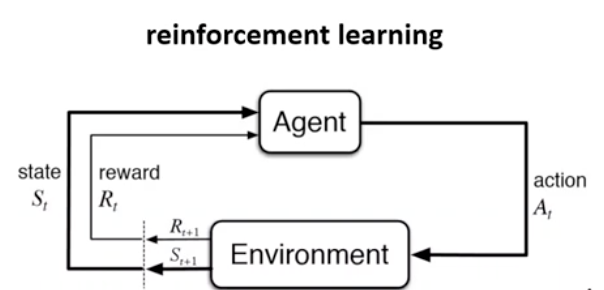
\includegraphics[scale=0.6]{./images/rl.png}
\end{center}

\noindent Reinforcement learning is about learning from interaction how to behave in order to achieve a goal. 
The reinforcement learning agent and its environment interact over a sequence of discrete time steps. 
The specification of their interface defines a particular task: the actions are the choices made by the agent; 
the states are the basis for making the choices; and the rewards are the basis for evaluating the choices. 
Everything inside the agent is completely known and controllable by the agent; 
everything outside is incompletely controllable but may or may not be completely known. 
A policy is a stochastic rule by which the agent selects actions as a function of states. 
The agent's objective is to maximize the amount of reward it receives over time.

\begin{itemize}
    \item There is no supervisor, only a reward signal
    \item Feedback is delayed, not instantaneous
    \item Time really matters (sequential, non independently identity distributed data)
    \item Agent’s actions affect the subsequent data it receives
\end{itemize}

\noindent Reinforcement learning is based on the reward hypothesis: 
All goals can be described by the maximisation of expected cumulative reward. 
The goal is select actions to maximise total future reward. 
Actions may have long term consequencesn, and reward may be delayed. 
It may be better to sacrifice immediate reward to gain more long-term reward.

\bigskip

\noindent The agent always learns to maximize its reward. 
If we want it to do something for us, we must provide rewards to it in such a way that in maximizing them the agent will also achieve our goals. 
It is thus critical that the rewards we set up truly indicate what we want accomplished. 
In particular, the reward signal is not the place to impart to the agent prior knowledge about how to achieve what we want it to do. 
If achieving subgoals were rewarded, then the agent might find a way to achieve them without achieving the real goal. 
The reward signal is your way of communicating to the agent what you want it to achieve, not how you want it achieved. 

\bigskip

\noindent \textbf{RL process}:

\begin{itemize}
    \item sample the trajectory (i.e. run the policy) in the environment
    \item estimate the performance of the policy
    \item improve the policy performance
    \item repeat
\end{itemize}

\noindent \textbf{RL algorithm categories}:

\begin{itemize}
    \item Value Based
    \begin{itemize}
        \item No Policy (Implicit)
        \item Have Value Function
    \end{itemize}
    \item Policy Based
    \begin{itemize}
        \item Have Policy
        \item No Value Function
    \end{itemize}
    \item Actor Critic
    \begin{itemize}
        \item Have Policy
        \item Have Value Function
    \end{itemize}
    \item Model Free
    \begin{itemize}
        \item Have Policy and/or Value Function
        \item No Model
    \end{itemize}
    \item Model Based
    \begin{itemize}
        \item Have Policy and/or Value Function
        \item Have Model
    \end{itemize}
\end{itemize}

\noindent \textbf{Learning vs Planning}:

\noindent There are two fundamental approaches in sequential decision making:

\begin{itemize}
    \item Reinforcement Learning
    \begin{itemize}
        \item The environment is initially unknown
        \item The agent interacts with the environment
        \item The agent improves its policy
    \end{itemize}
    \item Planning
    \begin{itemize}
        \item A model of the environment is known
        \item The agent performs computations with its model (without any external interaction)
        \item The agent improves its policy
        \item a.k.a. deliberation, reasoning, introspection, pondering, thought, search
    \end{itemize}
\end{itemize}

\noindent \textbf{Exploration vs Exploitation}:

\noindent Reinforcement learning is like trial-and-error learning. The agent should discover a good policy from its experiences of the environment, without losing too much reward along the way. 
It is usually important to explore as well as exploit.

\begin{itemize}
    \item Exploration
    \begin{itemize}
        \item finds more information about the environment
    \end{itemize}
    \item Exploitation
    \begin{itemize}
        \item exploits known information to maximise reward
    \end{itemize}
\end{itemize}

\noindent \textbf{Prediction vs Control}:

\begin{itemize}
    \item Prediction
    \begin{itemize}
        \item Given a policy, evaluate the future
    \end{itemize}
    \item Control
    \begin{itemize}
        \item Find the best policy, optimise the future
    \end{itemize}
\end{itemize}

\subsection{Summary of Notation}

\noindent \(\mathcal{S}\): set of all nonterminal states. \(\mathcal{S^+}\) represents set of all states including the terminal state.

\noindent \(\mathcal{A}\): set of all actions. \(\mathcal{A}(s)\) represents set of all actions available in state \(s\).

\noindent \(\mathcal{R}\): set of all possible rewards.

\noindent \(t\): discrete time step. \(t = 0, 1, 2, 3, \dots\).

\noindent \(O_t\): (not fully observed) observation of environment at time step \(t\).

\noindent \(A_t\): action at time step \(t\). \(A_t \in \mathcal{A}\).

\noindent \(S_t\): (fully observed) state of environment at time step \(t\). \(S_t \in \mathcal{S}\).

\noindent \(S_t^e\): environment state, the environment's private representation. 
Used by environment to pick the next observation/reward. 
The environment state is not usually visible to the agent, and may contain irrelevant information.

\noindent \(S_t^a\): agent state, the agent's internal representation of the environment. 
Used by agent to pick the next action. 
It is the state that used in RL algorithms. It can be a function of history: \(S_t^a = f(H_t)\). 
For example, it can be a complete history \(S_t^a = H_t\), 
or beliefs of environment state \(S_t^a = (P[S_t^e = s^1], \dots, P[S_t^e = s^n])\), 
or recurrent neural network \(S_t^a = \sigma(S_{t - 1}^a W_s + O_t W_o)\).

\noindent \textbf{Information state (Markov state)}: \(S_t\) that contains all useful information from the history. 
It is a compact summary of the history, which is as useful for predicting the future as the whole history. \(S_t = f(H_t)\). 
A state \(S_t\) is Markov if and only if: \(P[S_{t + 1} \mid S_t] = P[S_{t + 1} \mid S_1, \dots, S_t]\).

\noindent \(R_t\): reward at time step \(t\), typically due, stochastically, to \(S_{t - 1}\) and \(A_{t - 1}\). \(R_t \in \mathcal{R}\).

\noindent \(H_t\): history, a trajectory that contains a sequence of observations and actions up to time step \(t\). \(H_t = A_0, O_1, \dots, A_{t - 1}, O_{t}\).

\noindent \(\gamma\): discount factor. Determines the importance of future rewards, also to avoid infinite returns.

\noindent \(G_t\): return following time \(t\), the cumulative future reward. \(G_t = R_{t + 1} + \gamma R_{t + 2} + \gamma^2 R_{t + 3} + \dots\)

\noindent \(p(s', r \mid s, a)\): probability of transition to state \(s'\) with reward \(r\), from state \(s\) and action \(a\). It completely characterizes the environment's dynamics.

\[p(s', r \mid s, a) = Pr\{S_t = s', R_t = r | S_{t - 1} = s , A_{t - 1} = a \}\]
\[\sum_{s' \in \mathcal{S}} \sum_{r \in \mathcal{R}} p(s', r \mid s, a) = 1, \text{ for all \(s \in \mathcal{S}, a \in \mathcal{A}(s)\)}\]

\noindent \(p(s' \mid s, a)\): probability of transition to state \(s'\), from state \(s\) and action \(a\).

\[p(s' \mid s, a) = Pr\{S_t = s' | S_{t - 1} = s , A_{t - 1} = a \} = \sum_{r \in \mathcal{R}} p(s', r \mid s, a)\]

\noindent \(r(s, a)\): expected immediate reward from state \(s\) after action \(a\).

\[r(s, a) = E[R_t \mid S_{t - 1} = s , A_{t - 1} = a] = \sum_{r \in \mathcal{R}} r \sum_{s' \in \mathcal{S}} p(s', r \mid s, a)\]

\noindent \(r(s, a, s')\): expected immediate reward on transition from \(s\) to \(s'\) under action \(a\).

\[r(s, a, s') = E[R_t \mid S_{t - 1} = s , A_{t - 1} = a, S_t = s'] = \sum_{r \in \mathcal{R}} r p(r \mid s, a, s') = \sum_{r \in \mathcal{R}} r \frac{p(s', r \mid s, a)}{p(s' \mid s, a)}\]

\noindent \(\pi\): a policy decides agent's behaviour. It maps state to action. 
Deterministic policy: \(a = \pi(s)\). 
Stochastic policy: \(\pi(a \mid s) = P[A_t = a \mid S_t = s]\).

\noindent \(\pi_*\): optimal policy that gives best \(a\) for given \(s\).

\noindent \(v_{\pi}(s)\): value of state \(s\) under policy \(\pi\), estimates the expected return following state \(s\). 
For example, for discrete models it can be \(v_{\pi}(s) = E_{\pi}[G_t \mid S_t = s] = E_{\pi}[R_{t + 1} + \gamma R_{t + 2} + \gamma^2 R_{t + 3} + \dots \mid S_t = s]\).

\noindent \(v_{*}(s)\): value of state \(s\) under the optimal policy \(\pi_*\).

\noindent \(q_{\pi}(s, a)\): value of taking action a in state s under policy \(\pi\).

\noindent \(q_{*}(s, a)\): value of taking action \(a\) in state \(s\) under the optimal policy \(\pi_*\). Finding \(q_{*}(s, a)\) is the goal of RL tasks.

\noindent \(V\), \(V_t\): array estimates of state-value function \(v_{\pi}\) or \(v_{*}\).

\noindent \(Q\), \(Q_t\): array estimates of action-value function \(q_{\pi}\) or \(q_{*}\).

\noindent \(\bar{V}_{t}(s)\): expected approximate action value, e.g. \(\bar{V}_{t}(s) = \sum_a \pi(a \mid s) Q_t(s, a)\)

\noindent \(U_t\): target for estimate at time \(t\).

\section{Markov Chain and Markov Decision Process}

\subsection{Markov Chain}

\begin{center}
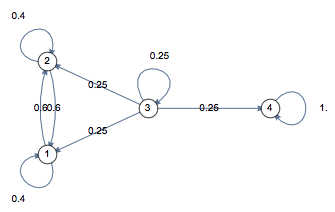
\includegraphics[scale=0.6]{./images/markov_chain_graph.png}
\end{center}

\noindent A Markov chain is a mathematical system that experiences transitions from one state to another according to certain probabilistic rules. The defining characteristic of a Markov chain is that no matter how the process arrived at its present state, the possible future states are fixed. In other words, the probability of transitioning to any particular state is dependent solely on the current state and time elapsed.

\subsection{Markov Decision Process}

\noindent MDPs are meant to be a straightforward framing of the problem of learning from interaction to achieve a goal. 
The learner and decision maker is called the agent. The thing it interacts with, comprising everything outside the agent, 
is called the environment. These interact continually, the agent selecting actions and the environment responding to these actions and presenting new situations to the agent. 
The environment also gives rise to rewards, special numerical values that the agent seeks to maximize over time through its choice of actions. 
The MDP and agent together thereby give rise to a sequence or trajectory that begins like this: \(S_0, A_0, R_1, S_1, A_1, R_2, \dots\). 
We use \(R_{t + 1}\) instead of \(R_t\) to denote the reward due to \(A_t\) because it emphasizes that the next reward and next state, \(R_{t + 1}\) and \(S_{t + 1}\), are jointly determined.


\bigskip

\noindent For episodic tasks, there is a finite time step \(T\) when a terminal state is reached. 
While for continuing tasks, there is not a terminal state and in this case \(T = \infty\). 
These two can be unified by considering episode termination to be the entering of a special absorbing state that transitions only to itself and that generates only rewards of zero.

\begin{center}
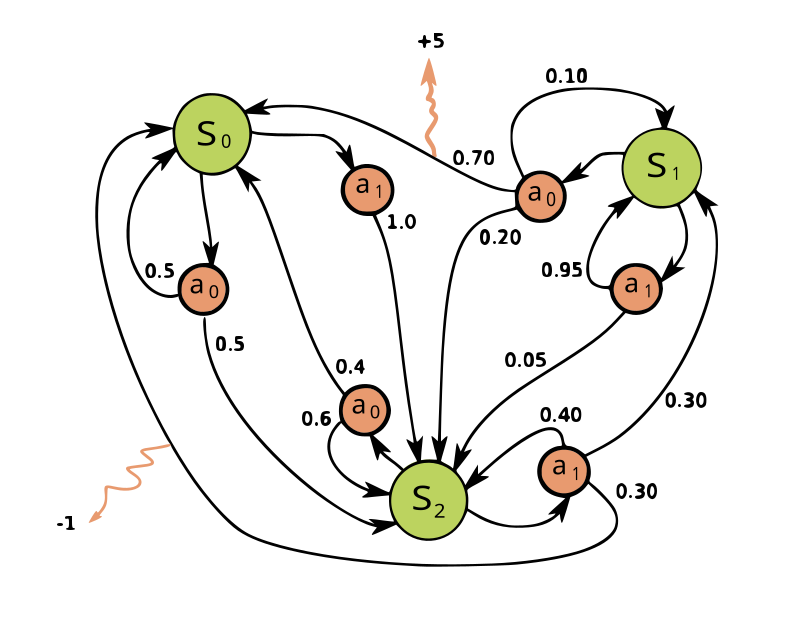
\includegraphics[scale=0.3]{./images/markov_decision_process.png}
\end{center}

\noindent Markov decision processes formally describe an environment for reinforcement learning. Where the environment is fully observable. 
The current state \(S_t\) completely characterises the process. "The future is independent of the past given the present". Almost all RL problems can be formalised as MDPs, e.g.

\begin{itemize}
    \item Optimal control primarily deals with continuous MDPs
    \item Partially observable problems can be converted into MDPs
    \item Bandits are MDPs with one state
\end{itemize}

\noindent A state \(S_t\) is Markov if and only if:

\[P[S_{t + 1} \mid S_t] = P[S_{t + 1} \mid S_1, \dots, S_t]\]

\bigskip

\noindent \(G_t\): the return \(G_t\) is the total discounted reward from time-step \(t\). Note here \(T = \infty\) or \(\gamma = 1\) is possible (but not both, otherwise return would be infinite).

\begin{equation*}
\begin{split}
G_t
& = R_{t + 1} + \gamma R_{t + 2} + \gamma^2 R_{t + 3} + \dots \\
& = \sum_{k = 0}^{T} \gamma^{k} R_{t + k + 1} \\
& = R_{t + 1} + \gamma G_{t + 1}
\end{split}
\end{equation*}

\noindent \(v_{\pi}(s)\): state-value function for policy \(\pi\), the expected return when starting in \(s\) and following \(\pi\) thereafter

\begin{equation*}
\begin{split}
v_{\pi}(s)
& = E_{\pi}[G_t \mid S_t = s] \\
& = E_{\pi}[R_{t + 1} + \gamma G_{t + 1} \mid S_t = s] \\
& = E_{\pi}[R_{t + 1} \mid S_t = s] + \gamma E_{\pi}[G_{t + 1} \mid S_t = s] \\
& = \sum_{a} \pi(a \mid s) E_{\pi}[R_{t + 1} \mid S_t = s, A_t = a] + \gamma \sum_{s'} p(s' \mid s) E_{\pi}[G_{t + 1} \mid S_{t + 1} = s'] \\
& = \sum_{a} \pi(a \mid s) r(s, a) + \gamma \sum_{s'} p(s' \mid s) v_{\pi}(s') \\
& = \sum_{a} \pi(a \mid s) \sum_r r \sum_{s'} p(s', r \mid s, a) + \gamma \sum_{s'} \sum_{a} \pi(a \mid s) p(s' \mid s, a) v_{\pi}(s') \\
& = \sum_{a} \pi(a \mid s) \sum_r r \sum_{s'} p(s', r \mid s, a) + \gamma \sum_{s'} \sum_{a} \pi(a \mid s) \sum_{r} p(s', r \mid s, a) v_{\pi}(s') \\
& = \sum_a \pi(a \mid s) \sum_{s', r} p(s', r \mid s, a) [r + \gamma v_{\pi}(s')]
\end{split}
\end{equation*}

\begin{equation*}
\begin{split}
v_{\pi}(s)
& = E_{\pi}[G_t \mid S_t = s] \\
& = E_{\pi}[R_{t + 1} + \gamma G_{t + 1} \mid S_t = s] \\
& = E_{\pi}[R_{t + 1} \mid S_t = s] + \gamma E_{\pi}[G_{t + 1} \mid S_t = s] \\
& = E_{\pi}[R_{t + 1} \mid S_t = s] + \gamma \sum_{s'} p(s' \mid s) E_{\pi}[G_{t + 1} \mid S_{t + 1} = s'] \\
& = E_{\pi}[R_{t + 1} \mid S_t = s] + \gamma \sum_{s'} p(s' \mid s) E_{\pi}[E_{\pi}[G_{t + 1} \mid S_{t + 1} = s'] \mid S_{t + 1} = s'] \\
& = E_{\pi}[R_{t + 1} \mid S_t = s] + \gamma E_{\pi}[E_{\pi}[G_{t + 1} \mid S_{t + 1} = s'] \mid S_t = s] \\
& = E_{\pi}[R_{t + 1} \mid S_t = s] + \gamma E_{\pi}[v_{\pi}(s') \mid S_t = s] \\
& = E_{\pi}[R_{t + 1} + \gamma v_{\pi}(s') \mid S_t = s]
\end{split}
\end{equation*}

\noindent \(q_{\pi}(s, a)\): action-value function for policy \(\pi\), the expected return starting from \(s\), taking the action \(a\), and following \(\pi\) thereafter

\begin{equation*}
\begin{split}
q_{\pi}(s, a)
& = E_{\pi}[G_t \mid S_t = s, A_t = a] \\
& = E_{\pi}[R_{t + 1} + \gamma G_{t + 1} \mid S_t = s, A_t = a] \\
& = E_{\pi}[R_{t + 1} \mid S_t = s, A_t = a] + \gamma E_{\pi}[G_{t + 1} \mid S_t = s, A_t = a] \\
& = r(s, a) + \gamma \sum_{s'} p(s' \mid s, a) E_{\pi}[G_{t + 1} \mid S_{t + 1} = s'] \\
& = \sum_r r \sum_{s'} p(s', r \mid s, a) + \gamma \sum_{s'} \sum_{r} p(s', r \mid s, a) \sum_{a'} \pi(a' \mid s') E_{\pi}[G_{t + 1} \mid S_{t + 1} = s', A_{t + 1} = a'] \\
& = \sum_r r \sum_{s'} p(s', r \mid s, a) + \gamma \sum_{s'} \sum_{r} p(s', r \mid s, a) \sum_{a'} \pi(a' \mid s') q_{\pi}(s', a') \\
& = \sum_{s', r} p(s', r \mid s, a) [r + \gamma \sum_{a'} \pi(a' \mid s') q_{\pi}(s', a')]
\end{split}
\end{equation*}

\begin{equation*}
\begin{split}
q_{\pi}(s, a)
& = E_{\pi}[G_t \mid S_t = s, A_t = a] \\
& = E_{\pi}[R_{t + 1} + \gamma G_{t + 1} \mid S_t = s, A_t = a] \\
& = E_{\pi}[R_{t + 1} \mid S_t = s, A_t = a] + \gamma E_{\pi}[G_{t + 1} \mid S_t = s, A_t = a] \\
& = E_{\pi}[R_{t + 1} \mid S_t = s, A_t = a] + \gamma \sum_{s', a'} p(s', a' \mid s, a) E_{\pi}[G_{t + 1} \mid S_{t + 1} = s', A_{t + 1} = a'] \\
& = E_{\pi}[R_{t + 1} \mid S_t = s, A_t = a] + \gamma \sum_{s', a'} p(s', a' \mid s, a) E_{\pi}[E_{\pi}[G_{t + 1} \mid S_{t + 1} = s', A_{t + 1} = a'] \mid S_{t + 1} = s', A_{t + 1} = a'] \\
& = E_{\pi}[R_{t + 1} \mid S_t = s, A_t = a] + \gamma E_{\pi}[E_{\pi}[G_{t + 1} \mid S_{t + 1} = s', A_{t + 1} = a'] \mid S_t = s, A_t = a] \\
& = E_{\pi}[R_{t + 1} \mid S_t = s, A_t = a] + \gamma E_{\pi}[q_{\pi}(s', a') \mid S_t = s, A_t = a] \\
& = E_{\pi}[R_{t + 1} + \gamma q_{\pi}(s', a') \mid S_t = s, A_t = a]
\end{split}
\end{equation*}

\noindent From the above equations, we can get following relationship between \(v_{\pi}(s)\) and \(q_{\pi}(s, a)\):

\begin{equation*}
\begin{split}
v_{\pi}(s)
& = E_{\pi}[G_t \mid S_t = s] \\
& = \sum_{a} \pi(a \mid s) E_{\pi}[G_t \mid S_t = s, A_t = a] \\
& = \sum_{a} \pi(a \mid s) q_{\pi}(s, a)
\end{split}
\end{equation*}

\begin{equation*}
\begin{split}
v_{\pi}(s)
& = E_{\pi}[G_t \mid S_t = s] \\
& = E_{\pi}[R_{t + 1} + \gamma G_{t + 1} \mid S_t = s] \\
& = E_{\pi}[R_{t + 1} \mid S_t = s] + \gamma E_{\pi}[G_{t + 1} \mid S_t = s] \\
& = E_{\pi}[R_{t + 1} \mid S_t = s] + \gamma \sum_{s', a'} p(s', a' \mid s) E_{\pi}[G_{t + 1} \mid S_{t + 1} = s', A_{t + 1} = a'] \\
& = E_{\pi}[R_{t + 1} \mid S_t = s] + \gamma \sum_{s', a'} p(s', a' \mid s) E_{\pi}[E_{\pi}[G_{t + 1} \mid S_{t + 1} = s', A_{t + 1} = a'] \mid S_{t + 1} = s', A_{t + 1} = a'] \\
& = E_{\pi}[R_{t + 1} \mid S_t = s] + \gamma E_{\pi}[E_{\pi}[G_{t + 1} \mid S_{t + 1} = s', A_{t + 1} = a'] \mid S_t = s] \\
& = E_{\pi}[R_{t + 1} \mid S_t = s] + \gamma E_{\pi}[q_{\pi}(s', a') \mid S_t = s] \\
& = E_{\pi}[R_{t + 1} + \gamma q_{\pi}(s', a') \mid S_t = s]
\end{split}
\end{equation*}

\begin{equation*}
\begin{split}
q_{\pi}(s, a)
& = E_{\pi}[G_t \mid S_t = s, A_t = a] \\
& = E_{\pi}[R_{t + 1} + \gamma G_{t + 1} \mid S_t = s, A_t = a] \\
& = E_{\pi}[R_{t + 1} \mid S_t = s, A_t = a] + \gamma E_{\pi}[G_{t + 1} \mid S_t = s, A_t = a] \\
& = r(s, a) + \gamma \sum_{s'} p(s' \mid s, a) E_{\pi}[G_{t + 1} \mid S_{t + 1} = s'] \\
& = \sum_r r \sum_{s'} p(s', r \mid s, a) + \gamma \sum_{s'} \sum_{r} p(s', r \mid s, a) v_{\pi}(s') \\
& = \sum_{s', r} p(s', r \mid s, a) [r + \gamma v_{\pi}(s')]
\end{split}
\end{equation*}

\begin{equation*}
\begin{split}
q_{\pi}(s, a)
& = E_{\pi}[G_t \mid S_t = s, A_t = a] \\
& = E_{\pi}[R_{t + 1} + \gamma G_{t + 1} \mid S_t = s, A_t = a] \\
& = E_{\pi}[R_{t + 1} \mid S_t = s, A_t = a] + \gamma E_{\pi}[G_{t + 1} \mid S_t = s, A_t = a] \\
& = E_{\pi}[R_{t + 1} \mid S_t = s, A_t = a] + \gamma \sum_{s'} p(s' \mid s, a) E_{\pi}[G_{t + 1} \mid S_{t + 1} = s'] \\
& = E_{\pi}[R_{t + 1} \mid S_t = s, A_t = a] + \gamma \sum_{s'} p(s' \mid s, a) E_{\pi}[E_{\pi}[G_{t + 1} \mid S_{t + 1} = s'] \mid S_{t + 1} = s'] \\
& = E_{\pi}[R_{t + 1} \mid S_t = s, A_t = a] + \gamma E_{\pi}[E_{\pi}[G_{t + 1} \mid S_{t + 1} = s'] \mid S_t = s, A_t = a] \\
& = E_{\pi}[R_{t + 1} \mid S_t = s, A_t = a] + \gamma E_{\pi}[v_{\pi}(s') \mid S_t = s, A_t = a] \\
& = E_{\pi}[R_{t + 1} + \gamma v_{\pi}(s') \mid S_t = s, A_t = a]
\end{split}
\end{equation*}

\noindent \(\pi_*\): the optimal policy (at least one, may be more than one). \(\pi \geq \pi'\) if and only if \(v_{\pi}(s) \geq v_{\pi'}(s)\) for all \(s \in \mathcal{S}\). 

\noindent \(v_*(s)\): the optimal state-value function, for all \(s \in \mathcal{S}\)

\[v_*(s) = \max_{\pi} v_{\pi}(s) \]

\noindent \(q_*(s, a)\): the optimal action-value function, for all \(s \in \mathcal{S}\) and \(a \in \mathcal{A}(s)\)

\[q_*(s, a) = \max_{\pi} q_{\pi}(s, a) \]

\noindent An optimal policy can be found by maximising over \(q_*(s, a)\):

\[
\pi_*(a \mid s) = 
\begin{cases}
1, & \text{if } a = \underset{a \in \mathcal{A}(s)}{\mathrm{argmax}} q_*(s, a) \\
0, & \text{otherwise}
\end{cases}
\]

\noindent All optimal policies achieve the optimal state-value function and the optimal action-value function, 
for all \(s \in \mathcal{S}\) and \(a \in \mathcal{A}(s)\)

\[v_{\pi_*}(s) = v_*(s) \]
\[q_{\pi_*}(s, a) = q_*(s, a) \]

\noindent The Bellman optimality equation for \(v_*\) intuitively expresses the fact that the value of a state under an optimal policy must equal the expected return for the best action from that state:

\begin{equation*}
\begin{split}
v_*(s)
& = \max_{a \in \mathcal{A}(s)} q_{\pi_*}(s, a) \\
& = \max_a E_{\pi_*}[G_t \mid S_t = s, A_t = a] \\
& = \max_a E_{\pi_*}[R_{t + 1} + \gamma G_{t + 1} \mid S_t = s, A_t = a] \\
& = \max_a E[R_{t + 1} + \gamma v_*(s') \mid S_t = s, A_t = a] \\
& = \max_a \sum_{s', r} p(s', r \mid s, a) [r + \gamma v_*(s')]
\end{split}
\end{equation*}

\noindent The Bellman optimality equation for \(q_*\), select the best action to maximize the future return:

\begin{equation*}
\begin{split}
q_*(s, a)
& = E[R_{t + 1} + \gamma \max_{a'} q_*(s', a') \mid S_t = s, A_t = a] \\
& = \sum_{s', r} p(s', r \mid s, a) [r + \gamma \max_{a'} q_*(s', a')]
\end{split}
\end{equation*}

\noindent For finite MDPs, the Bellman optimality equation is solvable. 
The Bellman optimality equation is actually a system of equations, one for each state, 
so if there are \(n\) states, then there are \(n\) equations in \(n\) unknowns. 
If the dynamics \(p\) of the environment are known, then in principle one can solve this system of equations for \(v_*\) using any one of a variety of methods for solving systems of nonlinear equations. 
One can solve a related set of equations for \(q_*\). 

\bigskip

\noindent Explicitly solving the Bellman optimality equation provides one route to finding an optimal policy, and thus to solving the reinforcement learning problem. 
However, this solution is rarely directly useful. It is akin to an exhaustive search, looking ahead at all possibilities, computing their probabilities of occurrence and their desirabilities in terms of expected rewards. 
This solution relies on at least three assumptions that are rarely true in practice: 

\begin{itemize}
    \item we accurately know the dynamics of the environment
    \item we have enough computational resources to complete the computation of the solution
    \item the Markov property
\end{itemize}

\noindent In reinforcement learning one typically has to settle for approximate solutions.

\section{Dynamic Programming}

\noindent The term dynamic programming (DP) refers to a collection of algorithms that can be used to compute optimal policies given a perfect model of the environment as a Markov decision process (MDP). 
Classical DP algorithms are of limited utility in reinforcement learning both because of their assumption of a perfect model and because of their great computational expense, but they are still important theoretically. 
DP provides an essential foundation for the understanding of the methods presented in the rest of this book. In fact, all of these methods can be viewed as attempts to achieve much the same eect as DP, 
only with less computation and without assuming a perfect model of the environment.

\bigskip

\noindent The key idea of DP, and of reinforcement learning generally, is the use of value functions to organize and structure the search for good policies. 
We can easily obtain optimal policies once we have found the optimal value functions, \(v_*\) or \(q_*\), which satisfy the Bellman optimality equations. 
As we shall see, DP algorithms are obtained by turning Bellman equations into assignments, that is, into update rules for improving approximations of the desired value functions.

\section{Imitation Learning}

\noindent Imitation learning, also known as learning from demonstration, is a process where an agent learns a new skill or behavior by observing and replicating the actions of others, often an expert. Training data are from expert inputs observations and actions. It assumes data is independently identity distributed, which is different from reinforcement learning. It is supervised learning.

\bigskip

\noindent \(p_{data}(o_t)\): Distribution of training data. The probability of taking action \(a_t\) at observation \(o_t\).

\noindent \(p_{\pi_{\theta}}(o_t)\): Distribution of validation data. The probability of taking correct action \(a_t\) at observation \(o_t\).

\noindent A standard training objective. Choose the optimal \(\theta\) that maxmizes the expectation of log probability of taking correct action \(a_t\) at observation \(o_t\), where \(o_t\) is sample from \(p_{data}(o_t)\):

\[\underset{\theta}{max} E_{o_t \sim p_{data}(o_t)}[log \pi_{\theta}(a_t \mid o_t)]\]
\[\underset{\theta}{max} \sum_{t = 1}^{m} log \pi_{\theta}(a_t \mid o_t)\]

\noindent An alternative training objective. We can either maxmize the reward:

\[r(o, a) = log p(a = \pi^*(o) \mid o)\]
\[\underset{\theta}{max} E_{o_t \sim p_{\pi_{\theta}}(o_t)}[r(o_t, a_t)]\]
\[\underset{\theta}{max} \sum_{t = 1}^{m} r(o_t, a_t)\]

\noindent Or, minimize the expect cost (number of mistakes) that the policy gonna make:

\[c(o_t, a_t) = 
\begin{cases}
0, & \text{if } a_t = \pi^*(o_t)\\
1, & \text{otherwise}
\end{cases}
\]
\[\underset{\theta}{min} E_{o_t \sim p_{\pi_{\theta}}(o_t)}[c(o_t, a_t)]\]
\[\underset{\theta}{min} \sum_{t = 1}^{m} c(o_t, a_t)\]

\noindent Imitation learning only learn from exsisting human behaviour, doesn't search for new approach. 
Sometimes the expert data is lacks of mistakes, after training the model can be trapped in an unfamiliar state and cannot recover from that it. 
Humans need to provide data, which is typically finite. Deep learning works best when data is plentiful, while humans are not good at providing some kinds of actions. 
So the result can hardly outperform humans'. Some approaches to improve performance:

\begin{itemize}
    \item Be smart about how we collect (and augment) our data.
    \begin{itemize}
        \item Intentionally add mistakes and corrections to training data. The mistakes hurt, but the corrections help, often more than the mistakes hurt.
        \item Use data augmentation. Add some "fake" data that illustrates corrections.
    \end{itemize}
    \item Use very powerful models that make very few mistakes.
    \begin{itemize}
        \item Mixture of gaussians.
        \item Latent variable models.
        \item Diffusion models.
    \end{itemize}
    \item Use multi-task learning. Learn \(\pi_{\theta}(a \mid o, g)\) instead. Add goal state \(g\) to the input. One good strategy is:
    \begin{itemize}
        \item Start with a random policy.
        \item Collect data with random goals.
        \item Treat this data as "demonstrations" for.
        \item the goals that were reached.
        \item Use this to improve the policy.
        \item Repeat.
    \end{itemize}
    \item Change the algorithm. DAgger (Dataset Aggregation) algorithm collects training data from \(p_{\pi_{\theta}}(o_t)\).
    \begin{itemize}
        \item Train \(\pi_{\theta}(a_t \mid o_t)\) from data (initially from human) \(D = \{(o_1, a_1), (o_2, a_2), \dots, (o_N, a_N)\}\).
        \item Run \(\pi_{\theta}(a_t \mid o_t)\) to get observation \(O_{\pi} = \{o_1, o_2, \dots, o_M\}\).
        \item Human labels them and get \(D_{\pi} = \{(o_1, a_1), (o_2, a_2), \dots, (o_M, a_M)\}\).
        \item Aggregate \(D = D \cup D_{\pi}\)
        \item Repeat.
    \end{itemize}
\end{itemize}

\section{Q-learning}

\noindent For any finite Markov decision process (FMDP), Q-learning finds an optimal policy in the sense of maximizing the expected value of the total reward over any and all successive steps, starting from the current state. Q-learning can identify an optimal action-selection policy for any given FMDP, given infinite exploration time and a partly-random policy.

\bigskip

\noindent \(s\): current state.

\noindent \(a\): current action.

\noindent \(s'\): new state after taking action \(a\).

\noindent \(a'\): action chosen on state \(s'\).

\noindent \(\gamma\): discount factor.

\noindent \(\eta\): soft update factor.

\noindent \(episode\): a sequence of states, from an initial state to a terminal state.

\noindent \(experience\): agent's experience on a state \((s, a, R(s), s')\).

\noindent \(M\): number of episodes.

\noindent \(T\): maximum episode length (time steps) if episode doesn't terminate.

\noindent \(N\): memory buffer capacity to store experiences.

\noindent \(C\): number of time steps for update.

\noindent \(B\): batch size.

\noindent \(R(s)\): reward from state \(s\).

\noindent \(\epsilon\): greedy policy during training - with probability \(\epsilon\), pick an action randomly; with probability \(1 - \epsilon\), pick the action that maximizes \(Q(s, a)\). (can start high and reduce gradually during the training process)

\bigskip

\noindent \(Q(s, a)\): The expected cumulative reward for taking action \(a\) on state \(s\), then choosing actions for the following states that maximizes cumulative reward.

\[Q(s, a) = R(s) + \gamma \max_{a'} Q(s', a')\]

\noindent \(\pi(s)\): a policy that given state \(s\), returns best action that maximizes the cumulative reward from state \(s\) onward.

\[\pi(s) = \underset{a}{argmax} \ Q(s, a)\]

\noindent \textbf{Training data}: get \((s_{i}, a_{i}, R(s_{i}), s_{i+1})\) experience tuple from environment.

\[x^{(i)} = s_{i}\]
\[
y^{(i)} =
\begin{cases}
  R(s_{i}), & \text{for terminal } s_{i+1} \\
  R(s_{i}) + \gamma \ \underset{a_{i+1}}{max} \ Q(s_{i+1}, a_{i+1}), & \text{for non-terminal } s_{i+1}
\end{cases}
\]

\noindent \textbf{Cost function}:

\[J(w, b) = \frac{1}{2m} \sum_{i = 1}^m (Q(s_{i}, a_{i}) - y^{(i)})^2\]

\noindent \textbf{Random (stochastic) environment?}

\noindent In a stochastic environment, after taking an action, the next state can have multiple possibilities. For example, after taking action \(a\), there is 0.1 chance that we get state \(s_1\), 0.2 chance to get state \(s_2\), and 0.7 chance to get state \(s_3\). To solve this problem, we can take the expectation of following cumulative reward:

\[Q(s, a) = R(s) + \gamma E[\max_{a'} Q(s', a')]\]

\noindent \textbf{Learning Process}:

\begin{center}
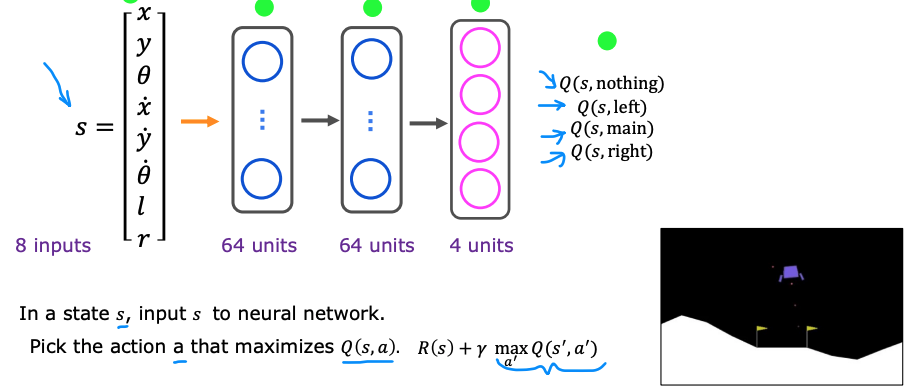
\includegraphics[scale=0.3]{./images/q_learning_nn.png}
\end{center}

\noindent Initialize memory buffer with capacity \(N\).

\noindent Initialize Q-network with random \(w, b\) as a guess of \(Q(s, a)\).

\noindent for \(i \in \{1, \dots, M\}\):

\noindent \hspace{.5cm} Receive initial state \(s_1\).

\noindent \hspace{.5cm} for \(t \in \{1, \dots, T\}\):

\noindent \hspace{1cm} Choose \(a_{t}\) for \(s_{t}\) with greedy policy \(\epsilon\).

\noindent \hspace{1cm} Get \((s_{t}, a_{t}, R(s_{t}), s_{t+1})\) experience tuple from environment.

\noindent \hspace{1cm} Store experience tuple in memory buffer, first in first out.

\bigskip

\noindent \hspace{1cm} Every \(C\) time steps perform a learning update:

\noindent \hspace{1cm} Sample \(B\) random experiences from memory buffer.

\noindent \hspace{1cm} For \((s_{j}, a_{j}, R(s_{j}), s_{j+1})\), \(j \in \{1, \dots, B\}\), construct training sample:

\[x^{(j)} = s_{j}\]
\[
y^{(j)} =
\begin{cases}
  R(s_{j}), & \text{for terminal } s_{j+1} \\
  R(s_{j}) + \gamma \ \underset{a_{j+1}}{max} \ Q(s_{j+1}, a_{j+1}), & \text{for non-terminal } s_{j+1}
\end{cases}
\]

\noindent \hspace{1cm} Train \(Q_{new}\) such that \(Q_{new}(s, a) \approx y\):

\noindent \hspace{1cm} Perform a gradient descent with mini batch and implement soft update:

\[w = (1 - \eta)w + \eta w_{new}\]
\[b = (1 - \eta)b + \eta b_{new}\]

\bigskip

\noindent \hspace{1cm} Start a new episode if \(s_{t+1}\) terminates, else continue.

\section{Policy Gradient}

\noindent \textbf{On-policy vs Off-policy learning}:

\noindent The key difference lies in how these methods approach learning:

\begin{itemize}
    \item On-policy:
    \begin{itemize}
        \item Training data is only generated from the exact same policy. e.g. Policy Gradient
        \item Learn from your own current strategy (even if it's not the best one yet).
    \end{itemize}
    \item Off-policy:
    \begin{itemize}
        \item Training data can originate from other sources that are not from the exact same policy. e.g. Q-learning, with greedy policy \(\epsilon\) in training, without \(\epsilon\) in prediction
        \item Learn from a different strategy (potentially better or more informed) than what you're currently using.
    \end{itemize}
    \item The primary distinction lies in how they approach exploration and exploitation, which affects their convergence properties and practical performance in different types of environments.
\end{itemize}

\noindent \textbf{Policy Gradient Algorithms}:

\noindent TBD: https://lilianweng.github.io/posts/2018-04-08-policy-gradient/

\section{Monte Carlo tree search (MCTS)}

\noindent The focus of MCTS is on the analysis of the most promising moves, expanding the search tree based on random sampling of the search space. The application of Monte Carlo tree search in games is based on many playouts, also called roll-outs. In each playout, the game is played out to the very end by selecting moves at random. The final game result of each playout is then used to weight the nodes in the game tree so that better nodes are more likely to be chosen in future playouts.

\bigskip

\noindent The most basic way to use playouts is to apply the same number of playouts after each legal move of the current player, then choose the move which led to the most victories. The efficiency of this method—called Pure Monte Carlo Game Search—often increases with time as more playouts are assigned to the moves that have frequently resulted in the current player's victory according to previous playouts. Each round of Monte Carlo tree search consists of four steps:

\begin{itemize}
    \item Selection: Start from root \(R\) and select successive child nodes until a leaf node \(L\) is reached. The root is the current game state and a leaf is any node that has a potential child from which no simulation (playout) has yet been initiated. \(L = R\) at the beginning of the search. The section below says more about a way (UCT) of biasing choice of child nodes that lets the game tree expand towards the most promising moves, which is the essence of Monte Carlo tree search.
    \item Expansion: Unless \(L\) ends the game decisively (e.g. win/loss/draw) for either player, create one (or more) child nodes. Child nodes are any valid moves from the game position defined by \(L\).
    \item Simulation: For each node \(C\) from the expanded nodes, complete one random playout from node \(C\). This step is sometimes also called playout or rollout. A playout may be as simple as choosing uniform random moves until the game is decided (for example in chess, the game is won, lost, or drawn).
    \item Backpropagation: Use the result of the playout to update information in the nodes on the path from \(C\) to \(R\).
\end{itemize}

\begin{center}
    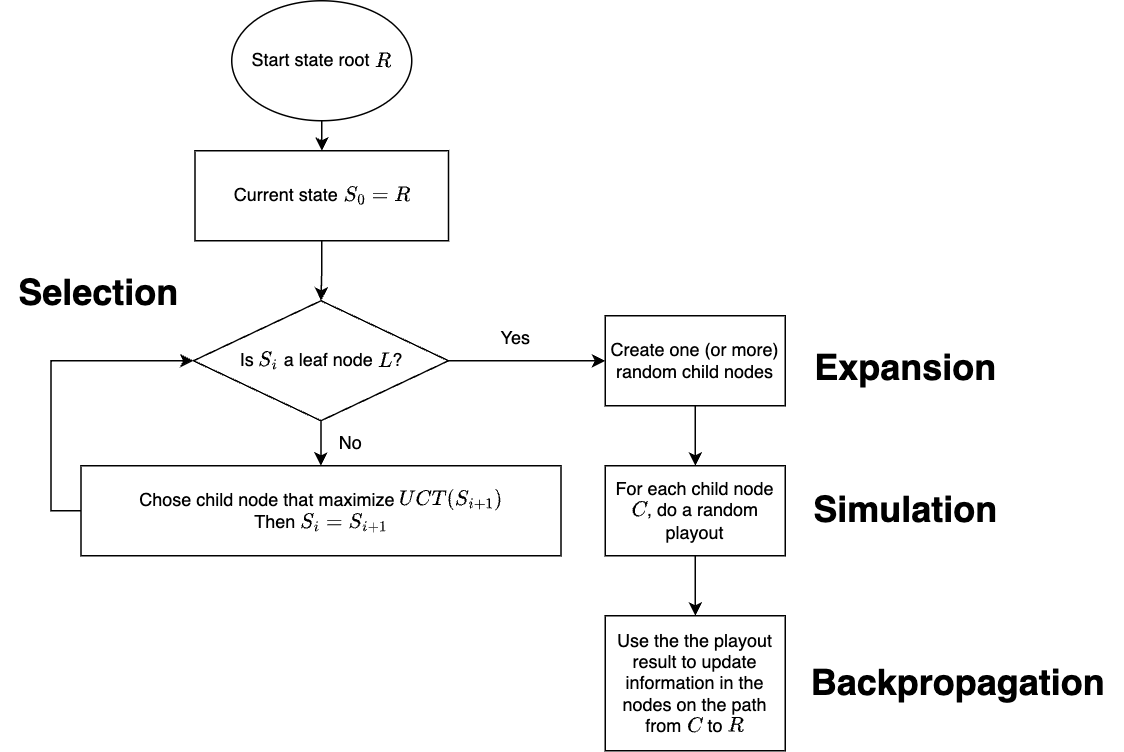
\includegraphics[scale=0.2]{./images/mcts_flow.png}
\end{center}

\begin{center}
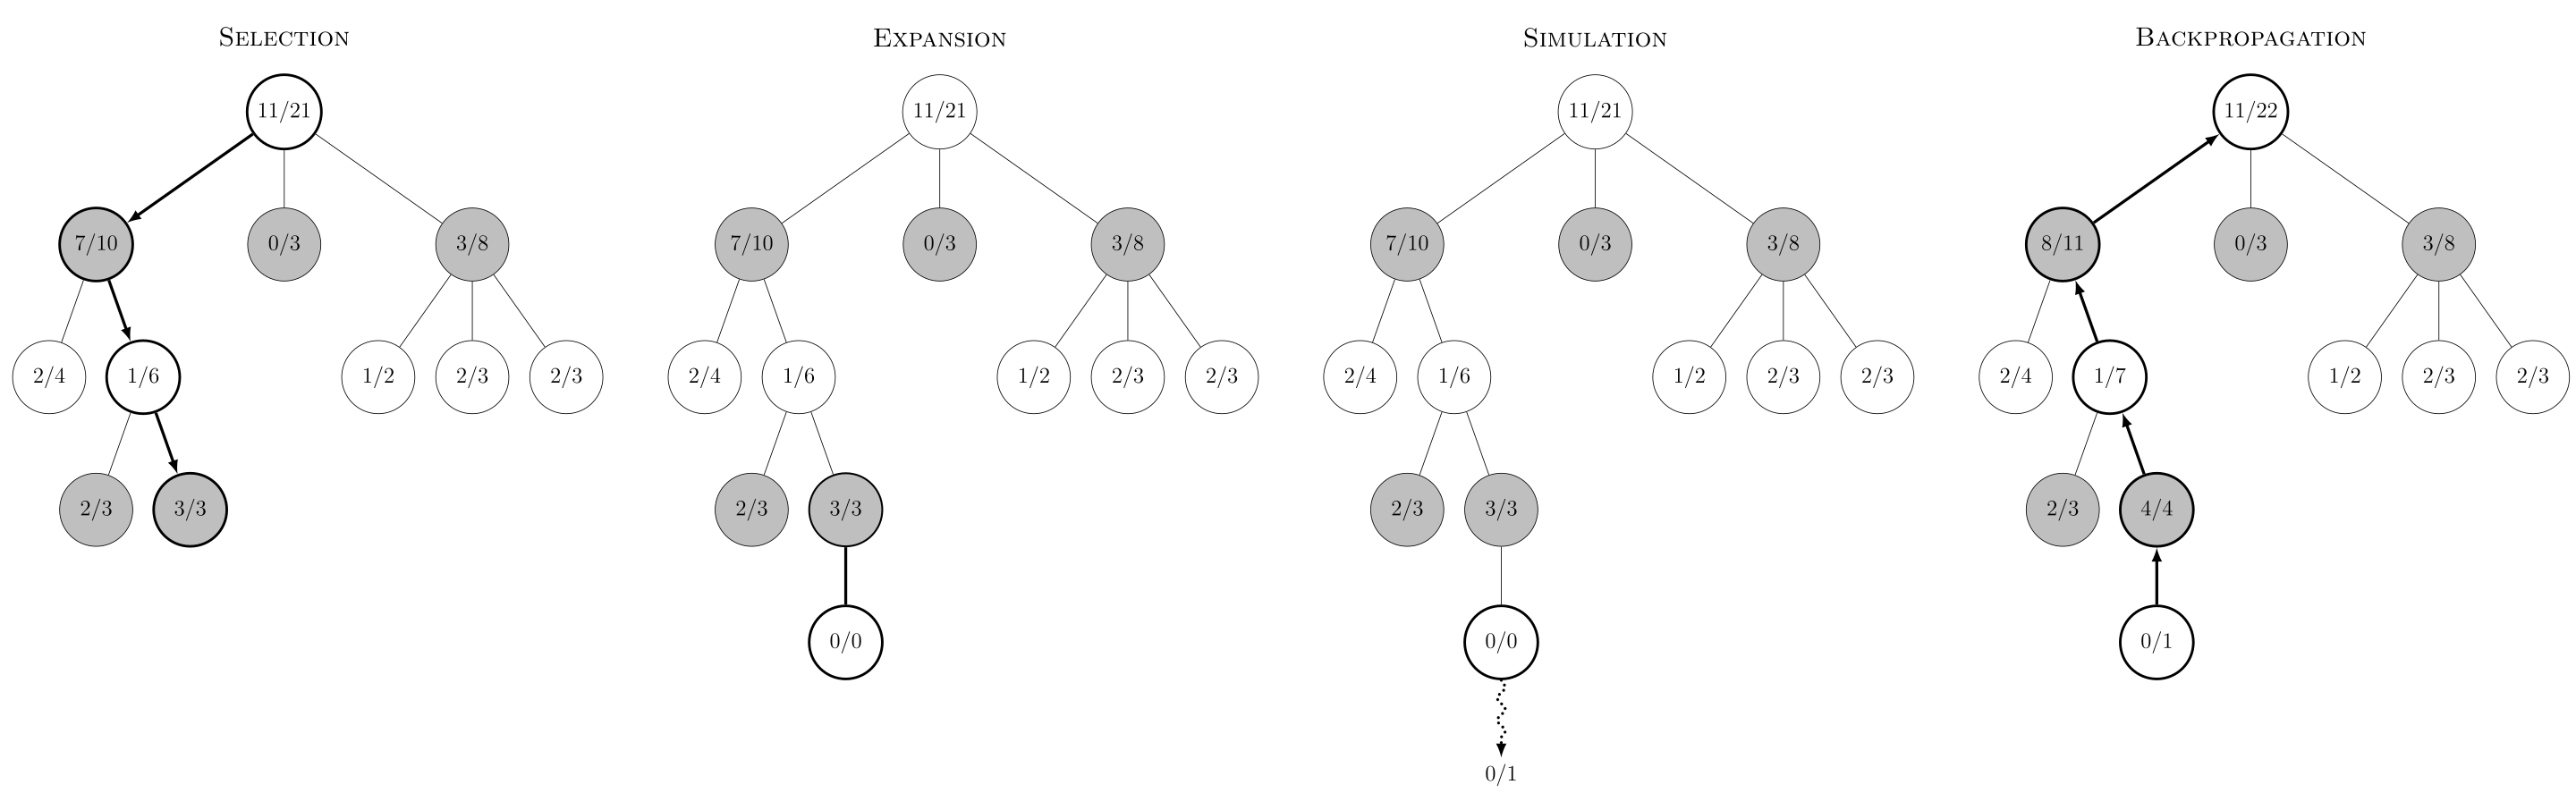
\includegraphics[scale=0.1]{./images/mcts_steps.png}
\end{center}

\noindent This graph shows the steps involved in one decision, with each node showing the ratio of wins to total playouts from that point in the game tree for the player that the node represents. In the Selection diagram, black is about to move. The root node shows there are 11 wins out of 21 playouts for white from this position so far. It complements the total of 10/21 black wins shown along the three black nodes under it, each of which represents a possible black move. Note that this graph does not follow the UCT algorithm described below.

\bigskip

\noindent If white loses the simulation, all nodes along the selection incremented their simulation count (the denominator), but among them only the black nodes were credited with wins (the numerator). If instead white wins, all nodes along the selection would still increment their simulation count, but among them only the white nodes would be credited with wins. In games where draws are possible, a draw causes the numerator for both black and white to be incremented by 0.5 and the denominator by 1. This ensures that during selection, each player's choices expand towards the most promising moves for that player, which mirrors the goal of each player to maximize the value of their move.

\bigskip

\noindent Rounds of search are repeated as long as the time allotted to a move remains. Then the move with the most simulations made (i.e. the highest denominator) is chosen as the final answer.

\bigskip

\noindent DeepMind's AlphaZero replaces the simulation step with an evaluation based on a neural network.

\bigskip

\noindent \textbf{UCT (Upper Confidence Bound 1 applied to trees):}

\bigskip

\noindent The main difficulty in selecting child nodes is maintaining some balance between the exploitation of deep variants after moves with high average win rate and the exploration of moves with few simulations. The first formula for balancing exploitation and exploration in games is called UCT. UCT recommends to choose in each node of the game tree the move for which the following expression has the highest value:

\[\frac{w_{i}}{n_{i}} + c \sqrt{\frac{ln N_{i}}{n_i}}\]

\begin{itemize}
    \item \(w_{i}\) stands for the number of wins for the node considered after the i-th move
    \item \(n_{i}\) stands for the number of simulations for the node considered after the i-th move
    \item \(N_{i}\) stands for the total number of simulations after the i-th move run by the parent node of the one considered
    \item \(c\) is the exploration parameter—theoretically equal to \(\sqrt{2}\); in practice usually chosen empirically
\end{itemize}

\noindent The first component of the formula above corresponds to exploitation; it is high for moves with high average win ratio. The second component corresponds to exploration; it is high for moves with few simulations.

\printindex

\end{document}